\documentclass[a4paper,12pt,twoside]{jreport}
\usepackage[T1]{fontenc} % Use T1 encoding (8bit font encoding)
\usepackage{lmodern} % Use Latin Modern (LM) font
%\usepackage{graphicx}
%\usepackage[dvips]{graphicx}
\usepackage[dvipdfmx]{graphicx}
\usepackage{longtable}
\usepackage{caption}
\usepackage{float}
\usepackage{kit-is-m}

%%===================================================================================
%% 一般情報 GENERAL INFORMATION
%% Overleaf を使用している場合は、Overleaf のデフォルト コンパイラ「pdfLaTeX」を「LaTeX」に切り替えます。
%% 「Menu -> Settings -> Compiler」でコンパイラを切り替えることができます。
%% If you are using Overleaf switch Overleaf's default compiler "pdfLaTeX" to "LaTeX".
%% You can do this under "Menu -> Settings -> Compiler"
%% 日本語テンプレートを使用するには、\EngCover を 0 に設定します。
%% Set \EngCover to 1 to use English template.
\EngCover{1}
\author{キッチケート キアラ}
\idnumber{23622999}
\deadline{2025}{2}{10} % 提出日{西暦年}{月}{日}(Date of submission, Feb. 8, 2024)
%% 長いタイトルで途中改行する場合,改行したい位置で

%%===================================================================================
%% 日本語設定 JAPANESE SETUP
%% \eauthor または \eauthori のどちらかを使うこと.
%% 日本人学生: 名-姓の順で定義する.
\eauthor{Taro}{Kosen} % 日本人学生のみ(名-姓の順であることに注意!) for Japanese students only
%% \coverbreak, \abstbreak, \\ のいずれかを使う.
%%   \coverbreak :表紙でのみこの位置で改行
%%    \abstbreak :概要でのみこの位置で改行
%%            \\ :表紙・概要ともにこの位置で改行
%%【例】
% \title{長い長いタイトル\coverbreak の改行位置\abstbreak に関する研究}
\title{修士論文・卒業研究報告書の書き方}
%% 以下,指導教員名の前の数字は職名を表す(順序ではない)
%% 1:教授,2:准教授,3:講師,4:助教,5:助手,
%% 6:特任教授,7:特任准教授,8:特任講師,9:特任助教,
%% 10:特定教授,11:特定准教授,12:特定講師,13:特定助教
%\advisor{1}{工繊 一郎} % 主任指導教員(工繊一郎教授)
%\secondadvisor{2}{情報 次郎} % (必要ならば)指導教員(情報次郎准教授)
%\thirdadvisor{4}{情報 三郎} % (必要ならば)指導教員(情報三郎助教)

%%===================================================================================
%% ENGLISH SETUP 英語設定
%% International students: Use \eauthori macro ONLY (DO NOT USE \eauthor macro. You must comment it out).
\eauthori{Chiara KITICAT} % for International students
%%        Write first and last names exactly as shown on your residence card.
%% If you want to break a line in the middle of a long title, use either \coverbreak, \abstbreak or \\.
%%   \coverbreak :line break here in coverpage only
%%    \abstbreak :line break here in abstract only
%%            \\ :line break here in both coverpage and abstract page
% \etitle{Very long title\coverbreak long long\abstbreak long title}
\etitle{How to write master's thesis or graduation report}
%% The first parameter describes a job title, not order.
%% 1:Prof., 2:Assoc.Prof., 3:Jr.Assoc.Prof., 4:Assist.Prof., 5: Assist.,
%% 6:Proj. Prof., 7:Proj. AP, 8:Proj. Jr. AP, 9:Proj. Assist.Prof.,
%% 10:Retd. Prof., 11:Retd. AP, 12:Retd. Jr. AP, 13:Retd. Assist.Prof.
\advisor{1}{Ichiro KOUSEN} % Prof. Ichiro KOUSEN
\secondadvisor{2}{Jiro JOHO} % (if needed) Assoc. Prof. Jiro JOHO
%\thirdadvisor{4}{Saburo JOHO} % (if needed) Assist. Prof. Saburo JOHO

%%===================================================================================
%% 論文の内容 THESIS CONTENT
\begin{document}
\maketitle

%%
%% 和文概要
%%
\begin{abstract}
Writing a master's thesis or a graduation research report is the culmination of master's and undergraduate studies, and its aims are to overview and systematize specialized knowledge, to develop logical writing skills, and to develop the ability to proceed with things planned under time constraints.

This document aims to explain the format and structure of a master's thesis or graduation research report, and to provide examples of how to write it. Since a master's thesis or graduation research report is equivalent to an academic paper, it is important that all assertions and evaluations are based on evidence. There is an appropriate way to write such a document that is easy for the reader to understand, but it is important to define the format and structure in order to avoid the waste of reinventing the wheel, which is to say, to devise a way to write it one's own way.

Regarding "format" that is not dependent on the content, such as booklet format, characters and terminology, mathematical formulas, figures, photographs, tables, and footnotes, in principle, the submission guidelines of the IEICE Japanese Journal D should be followed. It is acceptable to follow the submission guidelines of the Information Processing Society of Japan, but mixing with the IEICE guidelines is not permitted.

The structure of a paper or report should be in the following order: Japanese abstract, English abstract (master's thesis only), table of contents, main text + figures and tables, and appendix.
The main text should be written in the following order: Chapter 1 (Introduction), followed by the final chapter (Conclusion), Acknowledgements, and References.

The abstract should be concise and clear, within one page, and should not cite any specific symbols, formulas, figures, or diagrams that are explained in the main text, nor should it include any figures or tables. On the other hand, the introduction is not read on its own, so figures, formulas, letters, symbols, etc. in the main text may be quoted, and figures and tables may be included. The conclusion is part of the main text, so it should only summarize the research methods and results, without including the introduction, and should not include previous research or conventional methods presented in subsequent chapters. In the conclusion, write mainly about what was achieved, and briefly about what remains to be done, i.e., future challenges.

Derivations of mathematical formulas that are not directly related to the argument, detailed explanations of cited references, detailed experimental data, etc. should not be included in the main text, but should be written together at the end of the text as an appendix. Items that are not commonly read through, such as source code or data dump lists, should not be included in either the main text or the appendix.

When writing a paper or report, we recommend ensuring sufficient time for writing and sleep, eating regular meals in the morning, afternoon, and evening, quickly becoming proficient in \TeX, Word, etc., repeatedly self-revising, versioning the manuscript, and saving both the old and new files.
\end{abstract}

%%
%% 英文概要(150〜200 words)
%% English Abstract (150-200 words)
%%
%% 【注意】
%% このスタイルファイルが生成する英文概要は,学務課が要求する
%% 書式と厳密には一致しない.
%% 学務課へは別途 Word ファイル(Docx形式)の提出が必要なので,
%% Word 上で最終印刷することを勧める.
%% Please print out the final edition of the abstract by using MS Word 
%% for submitting to the Educational Affairs. You also have to submit 
%% the Word (docx) file online.
%\begin{eabstract}
%修士論文や卒業研究報告書の執筆は,修士および学部における学修の総仕上げで
%あり,そのねらいは,専門知識の俯瞰と体系化,論理的な文章の記述力養成,
%時間制約の下で計画的に物事を進める能力の養成,にある.
%本文書は,修士論文・卒業研究報告書の体裁や構成を説明し,書き方の見本を
%示すことを目的とする.
%修士論文や卒業研究報告書は,いわゆる学術論文に準ずるので,「全ての主張や
%評価が根拠に基づいている」こと が重要である.
%そのような文章には,読み手が把握しやすい適切な書き方があるが,それを各自
%勝手に工夫する,いわゆる車輪の再発明の無駄を避ける点で,体裁や構成を
%定める意義がある.
%冊子体裁,用字と用語,数式,図・写真・表,脚注など内容に依らない「体裁」
%については,原則として電子情報通信学会和文論文誌Dの投稿規定に準拠する.
%情報処理学会の投稿規定に準拠してもよいが,信学会規定との混在は認めない.
%論文や報告書の構成は,和文概要,英文概要(修士論文のみ),目次,本文+
%図表,付録の順とする.
%本文は,第1章緒言から最終章結言,謝辞,参考文献の順に書く.
%概要は,背景,目的,方法,結果,結論を簡潔明快に1ページ以内で記述し,
%本文中に説明のある特定の記号,数式,図表などを引用せず,図表も含めない.
%一方,緒言は単独では読まないので,本文中の図,式,文字,記号等を引用し
%てもよく,図表を含めてもよい.
%結言は本文の一部なので,研究方法と研究結果のみを要約し,緒言は含めず,
%続の章で示した先行研究や従来手法なども含めない.
%結言には,達成したことを主に書き,積み残したこと,すなわち今後の課題は
%簡潔に書く.
%論旨に直接関係ない数式の誘導,引用文献の詳解,実験の詳細なデータなどは,
%本文に書かず付録として本文の後ろにまとめて書く.
%ソースコードやデータのダンプリストなど,常識的に通読しないものは本文に
%も付録にも含めてはならない.
%論文や報告書の執筆にあたっては,十分な執筆時間と睡眠時間の確保,朝昼夕の
%規則正しい食事,\TeX, Word等の早期習熟,自己推敲の繰り返し,原稿の
%バージョン管理と新旧ファイル両方の保存を推奨する.
%\end{eabstract}

\begin{contents}
\tableofcontents % 目次の作成(Table of Contents)
%\nchapter{記号・略語一覧} % 必要ならば
%% ここに記号説明を書く
%\nchapter{Glossary} % if needed
%% Write here the explanation of symbols and abbreviations.
\end{contents}

\chapter{Introductions}
The purpose of this report is to provide examples of master's theses and graduation research reports. Writing a master's thesis or graduation research report is the culmination of master's or undergraduate studies, and its aims are to overview and systematize specialized knowledge, to develop logical writing skills, and to develop the ability to proceed with things in a planned manner under time constraints. These abilities are essential for active participation in society as an engineering professional, regardless of field.

I would like students to devote all their energy to writing reports and papers for the next step. Since master's theses and graduation research reports are equivalent to so-called academic papers, it is important that "all assertions and evaluations are based on evidence." "Based on evidence" means that assertions and evaluations are derived rationally from documents that can prove the existence of facts, such as literature, statistics, and experimental data. Assertions and evaluations that are not based on evidence are extremely unconvincing because others cannot verify their truthfulness, and are considered to be mere impressions. Students should always ask themselves, "What is the basis for my argument?" when writing a paper or report.

The purpose of writing a master's thesis or graduation research report, especially the format and structure, is to write appropriate sentences that are easy for the reader to understand. Our predecessors have reached a certain degree of consensus on how to write academic papers through a long process of trial and error. Writing style is a kind of intellectual property, and respecting it is meaningful in that it helps to avoid the waste of "reinventing the wheel," where each person tries to come up with appropriate sentences on their own. When you are not used to it, the detailed instructions on how to write may seem cumbersome, but this is often because there is no basis for your argument or evaluation, or you do not have enough time to write in the first place. We would like students to respect the instructions on how to write, which are the accumulation of the wisdom of our predecessors, and write with enough time to follow them.

Here is the structure of this report. First, we will explain the format of a thesis, which is independent of the content, such as booklet format, characters and terminology, mathematical formulas, figures, photographs, tables, and footnotes. Next, we will explain the structure, i.e. what to write and in what order. Finally, we will conclude by introducing recommended actions to take when writing a thesis or report while adhering to the format and structure. We will also provide examples of reference lists and appendices, as well as how to write bibliographic information and the requirements for submitting a master's thesis pdf file.

\chapter{Format of the Paper}
\section{Basics}
The format of the paper should, in principle, follow the submission guidelines of the Japanese journal D of the Institute of Electronics, Information and Communication Engineers (IEICE). It may be acceptable to follow the submission guidelines of the Information Processing Society of Japan, but mixing them with IEICE guidelines is not permitted. Matters specific to master's theses and graduation research reports should be based on this report.

\section{Booklet Format}
Details of the booklet format are shown in Table \ref{tab1}. The front and back covers and binding tape will be those distributed through the laboratory. For graduation research reports, only the bound booklet should be submitted, and pdf files etc. should not be submitted (these will be kept separately in the laboratory). For master's theses, both the thesis pdf file and the bound booklet should be submitted. If necessary, a zip file containing related data may be submitted. Thesis pdf files and zip files should be submitted to the designated Moodle course.

%\begin{table}[p]
%\begin{center}
%\caption{List of master's theses and graduation research reports in booklet format}
%\label{tab1}
%\begin{tabular}{p{5.5zw}|p{29zw}} \Hline
%Item & Content \\ \hline
%Format and shape & A4 portrait, horizontal writing \\ \hline
%Amount of text & In principle, the text should be at least 20 pages, excluding pages of figures and tables. \\ \hline
%Page settings & 37 full-width characters x 30 lines per page, single column, 25mm margins on all sides. \\ \hline
%Font & text should be 12pt, with chapter/section headings and cover page appropriately large in accordance with this report. \\ \hline
%Pagination (page numbers) & Place consecutive numbers only in the bottom center of the page. Do not use parentheses or hyphens. Do not use them on the cover or summary. Use Roman numerals (lowercase) for the table of contents (including symbol explanations), and use Arabic numerals from the beginning of the main text + figures and tables to the end of any appendices. \\ \hline
%Paper & front and back covers should be printed on colored high-quality paper (light blue for graduation research reports, light green for master's theses), and everything else should be printed on plain paper. \\ \hline
%Printing & Print in black and white as a rule. Cover and synopsis printed on one side. Everything else printed on both sides. If the table of contents is an odd number of pages, the back of the last table of contents page should be left blank with only the folio number, and the main text should be printed on new paper. There is no need to start chapters on odd-numbered pages, so do not insert blank pages in the main text. \\ \hline
%Binding & Staple the three left-hand sides, then cover them with binding tape from the fore-edge to create a simple binding. Avoid stapling in the two-hole punch position (center $\pm$ 40mm). Do not punch holes.\\ \Hline
%\end{tabular}
%\end{center}
%\end{table}

\begin{center}
\captionof{table}{List of master's theses and graduation research reports in booklet format}
\label{tab1}
\end{center}

\begin{longtable}{p{5.5zw}|p{29zw}}
%\caption{List of master's theses and graduation research reports in booklet format} \label{tab1} \\
\Hline
Item & Content \\ \hline
\endfirsthead

\Hline
Item & Content \\ \hline
\endhead

\hline
\endfoot

\Hline
\endlastfoot

Format and shape & A4 portrait, horizontal writing \\ \hline
Amount of text & In principle, the text should be at least 20 pages, excluding pages of figures and tables. \\ \hline
Page settings & 37 full-width characters x 30 lines per page, single column, 25mm margins on all sides. \\ \hline
Font & text should be 12pt, with chapter/section headings and cover page appropriately large in accordance with this report. \\ \hline
Pagination (page numbers) & Place consecutive numbers only in the bottom center of the page. Do not use parentheses or hyphens. Do not use them on the cover or summary. Use Roman numerals (lowercase) for the table of contents (including symbol explanations), and use Arabic numerals from the beginning of the main text + figures and tables to the end of any appendices. \\ \hline
Paper & front and back covers should be printed on colored high-quality paper (light blue for graduation research reports, light green for master's theses), and everything else should be printed on plain paper. \\ \hline
Printing & Print in black and white as a rule. Cover and synopsis printed on one side. Everything else printed on both sides. If the table of contents is an odd number of pages, the back of the last table of contents page should be left blank with only the folio number, and the main text should be printed on new paper. There is no need to start chapters on odd-numbered pages, so do not insert blank pages in the main text. \\ \hline
Binding & Staple the three left-hand sides, then cover them with binding tape from the fore-edge to create a simple binding. Avoid stapling in the two-hole punch position (center $\pm$ 40mm). Do not punch holes.\\
\end{longtable}

\section{Script and Terminology}
This section explains the characters and terminology\footnote{Quoted from the Guide to Submitting Papers to the Japanese Journal of the Institute of Electronics, Information and Communication Engineers (Information and Systems Society), 2.4 Characters and Terminology.}
\begin{itemize}
\item[(a)] In principle, the characters used are "common kanji" and kana are "new kana usage" (Appendix F)\footnote{http://www.ieice.org/jpn/shiori/pdf/furoku\_f.pdf}.
\item[(b)] In principle, the terms are
(1) "Ministry of Education Academic Glossary, Electrical Engineering Edition" and IEICE
(2) "Electronics, Information and Communication Terminology Dictionary",
(3) Based on the "Electronics, Information and Communications Handbook."
\item[(c)] In principle, the abbreviations (SI) and symbols of quantity symbols and unit symbols should be those in the "Electronics, Information and Communication Handbook" compiled by the IEICE.
\item[(d)] For punctuation, use the full-width period "." and comma ",".
\end{itemize}

\section{Formula}
Equations are typeset using \LaTeX display mode, Microsoft Office equation editor
(2D format), etc. Equations should be written on separate lines, centered or with equal sign alignment, as much as possible, without being embedded in the text. So-called inline formats, such as writing fractions as 1/2 or writing the upper and lower limits of a sum symbol to the right of $\Sigma$, should not be used. As shown in the formula (\ref{eqn1}), equation numbers in the format (chapter number.serial number) should be added to the right of each equation and cited in the main text.

\begin{equation}
y(n)=\sum_{k=-\infty}^{\infty}x(k)h(n-k)\label{eqn1}
\end{equation}

\section{Figures, Photographs, and Tables}
In principle, only figures, photographs (based on the figure), and tables created by the author should be used. Copying (scanning and pasting) from literature, books, the web, etc. is strictly prohibited. When quoting copyrighted material, be sure to clearly indicate the source and avoid infringing copyright.

Line drawings should be carefully drawn using drawing software such as PowerPoint, Illustrator, PiC\TeX, PSTricks, etc. Graphs should be created using Excel or Gnuplot, etc. Figures should have a title (caption) in the format Figure [chapter number]. [figure number within chapter] [figure caption] added to the bottom of the figure. When a figure contains multiple elements, such as Figure~\ref{fig1}, each element should have a sub-heading beginning with (a), (b), (c), ...

Tables must have column headers, and row headers should be added as necessary. Tables should have as few lines as possible. Do not draw vertical lines on the left or right edges. Use thick or double horizontal lines at the top and bottom. Tables should have a title in the format Table [chapter number]. [table number within chapter] [table header] at the top of the table.

The submission guidelines for IEICE Transactions on Japanese Language D state that English titles should be included with figures and tables, but English titles are not required for master's theses and graduation research reports.

Figures and tables should be drawn in monochrome, except in cases where color is required, such as color images or display screens. For example, when drawing multiple line graphs, distinguish each line by line type, rather than by color.

\section{Footnote}
If explaining in the main text would disrupt the context, write the explanation in a footnote. If the explanation is too long, put it in an appendix. For footnotes, draw a horizontal line at the bottom of the page and write (Note [Serial number (Arabic numerals)]): XXXXX underneath. (Note [Serial number]) should also be added in superscript to references in the main text.

If it is difficult to automatically number (Note [Serial number]) when typesetting in Word, it is better to use a method like this report \footnote{This has been typeset using \LaTeX, so it is a valid footnote.}. A format in which only consecutive numbers are given in superscript Arabic numerals at the left margin and in in-text note references may be used.

\chapter{Structure of the Paper}
\section{Front and Back Cover}
The cover has a picture \ref{fig1}. Write the contents shown in the above text centered. A receipt stamp will be affixed to the document, so be sure to avoid any typos. Do not print anything on the back cover.

\begin{figure}[p] % 図は必ず[p]で取り込むこと(You must include a figure using [p] option.)
\begin{center}
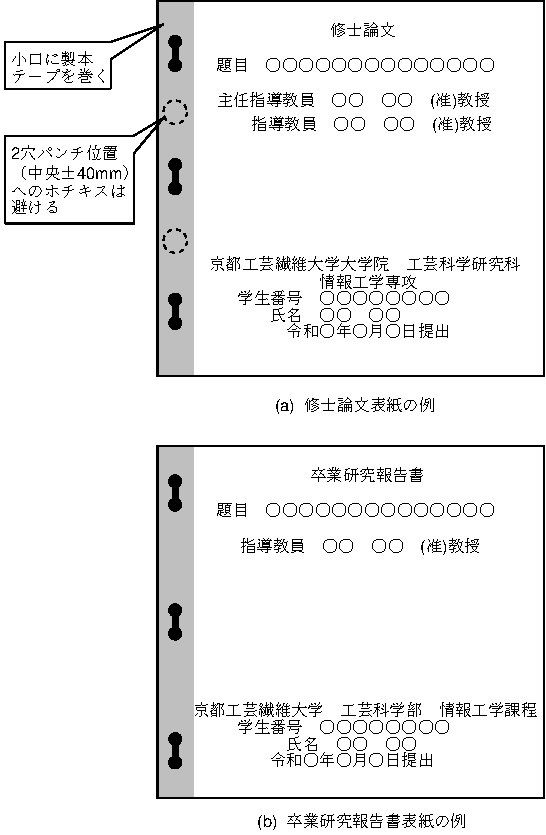
\includegraphics[scale=1.0]{assets/coverpage.pdf}
\caption{Examples of master's thesis and graduation research report covers}
\label{fig1} % \label は \caption の直後に付ける(The \label should be placed immediately after the \caption.)
\end{center}
\end{figure}

\section{Summary}
The Japanese abstract should be concise and clear on one page, describing the background, purpose, methods, results, and conclusion. Do not cite specific symbols, formulas, figures, tables, etc. that are explained in the main text. Figures and tables are not included. For both the master's thesis and graduation research report, write [Research title] on the first line, [Reiwa year xx month xx day (submission date)][Student number][Name] on the third line, and "Abstract" on the fifth line, and then write the abstract from the sixth line onward.

For master's thesis, the content should be basically the same as that of the "Thesis/Specific Subject Abstract (Japanese)" applied for on the Academic Affairs Office website. A seal is not required.

\section{Abstract in English (Master's thesis only)}
The content should be the same as that of the "Thesis/Specific Project Abstract (English)" submitted via the Academic Affairs Division website. Write [Research Title] on the first line, [Month Day, Year (submission date)][Student ID][Name] on the third line, and "Abstract" on the fifth line, and start writing the abstract from the sixth line. It does not need to be a literal translation of the Japanese abstract. The word count should follow the guidelines on the Academic Affairs Division website (150-200 words).

\section{Table of Contents}
Write "Table of Contents" on the first line, and from the third line onward, list the relevant pages for each chapter and section of the main text.

List the relevant pages for acknowledgments and appendices as well. If you are creating a page to explain and define all the symbols used in the main text, place this page immediately after the table of contents.

\section{Main text + figures and tables}
The main text consists of Chapter 1 (Introduction) through Chapter n (Conclusion), as well as the References and Acknowledgments. Anything after that is considered an appendix. Figures and tables should be treated as separate pages, and inserted immediately after the page on which they are first mentioned in the main text. It is acceptable to fit two or three figures and tables onto one page.

References should be cited in appropriate places in the main text, with numbers such as [12] in half-width characters. They should not be super-scripted. Use a new page when starting a new chapter, but it is not necessary to start a chapter on an odd-numbered page. Below is an explanation of what should be written where in the main text.

\begin{description}
\item[{\bfseries 1. Introduction} \\]
Explain the purpose of this study (what and to what extent it will be clarified), its position in the research field, its significance, the historical background, and an overview of previous research, and then list the structure of Chapter 2 and beyond (what will be stated in each chapter). Unlike an overview, the introduction is not read on its own, so you may quote figures, formulas, letters, symbols, etc. from the main text.

\item[{\bfseries 2. Chapter 2 to Chapter (n-1)}]
Divide the research methods and results into chapters to make them easy for readers to understand, and give them unique chapter headings. Each chapter should be further divided into sections with unique section headings. Number the chapters and sections as 2. (with a period), 2.1, 2.1.1, etc.

\item[{\bfseries 3. Chapter n Conclusion (Conclusion, Summary)}]
The outline summarizes the entire text, but the conclusion summarizes only the research methods and results, without including the introduction. It does not include previous research or conventional methods published in Chapters 2 to (n-1) for comparison with your own theory. Since the purpose is to summarize what has been achieved, what remains to be done (future challenges) will be written briefly.

\item[{\bfseries 4. Acknowledgments}]
Following the conclusion, start a new line (but do not start a page break) and express your gratitude to those who have guided you and those or organizations who have helped you (if your supervisor has instructed you to do so for research grants, etc.). To avoid disrespect, write the names of the people in full, and write their affiliations and titles accurately. Specific matters, such as the provision of data or samples, may be noted in footnotes.

\item[{\bfseries 5. References}]
List the bibliographic information of your references in the order they are cited in the text. The writing style is quoted below.\footnote{Cited from the IEICE Transactions on Japanese Language Submissions (Information and Systems Society) 2.6.1 List of References.}.
\begin{itemize}
\item[(a)] Appendix G: List of Academic Journal Abbreviations \footnote{http://www.ieice.org/jpn/shiori/pdf/furoku\_g.pdf}. The names of journals listed in the table will be abbreviated according to the same table.
\item[(b)] If there are multiple authors, write the names of all the authors. If the name is written in Western language, write the initials and the surname, and insert a half-width space only between the initials and the surname, such as A.G. Wine.
\item[(c)] Words in the title of an English paper should be in lowercase except for the first sentence.
\item[(d)] In Western documents, half-width periods (.) and half-width commas (,) are always used. In Japanese documents, full-width "," is used for commas, and half-width periods (.) are used for abbreviations such as "vol.", "no.", "pp.", and month names, and for full stops at the end of lines. Note that in the case of vol.J62-B, no.1, pp.20-27, etc., no space is inserted after the half-width period (.).
\item[(e)] When listing the publication date, use the order of month and year, with the month name in English and the year in the Gregorian calendar.
\item[(f)] References to the URL of the web page in question should be used effectively as necessary to clarify novelty, validity, and reliability, or to reinforce the argument. However, since third-party web pages are likely to be revised or deleted, refer to the original article whenever possible.
\end{itemize}

Table \ref{tab2} shows the format for a bibliography organized by document type.
\end{description}


\begin{table}[p]
\begin{center}
\caption{Reference Format}
\label{tab2}
\begin{tabular}{p{36mm}|p{105mm}} \Hline
Document types & Bibliographic formats\\ \hline
Magazine\cite{YY79}\cite{RWG64}
 & Author name, ``title,'' journal name, volume, issue, start-end pages with pp., month and year.\\ \hline
Books and Edited Books\cite{Y89}\cite{TON90}
 & Author name, book title, editor name, publisher, city of issue
City name, publication year.\\ \hline
When quoting part of a book\cite{YA89}\cite{HSR72}
 & Start-end with author name, "title," book title, editor name, chapter number or pp.
Page number, publisher, city of publication, year of publication.\\ \hline
International Conference\cite{YMI90}
 & Author name, title, conference name, paper number with no.,
   Start-end page number with pp., host city name, country name, month and year. \\ \hline
Domestic conference, research group papers\cite{KK95}
 & Author name, "Title," name of conference proceedings, volume or issue,
   Add no. to indicate the paper number, pp. to indicate the start-end page number, and month and year.\\\hline
electronic media\cite{KK79}
 & Author name, "title," journal name, volume, issue, start-end page numbers with pp.,
   Month and year (online), where to get it $\langle$ Reference Examples$\rangle$ , (reference date)
   \\\hline
Webpage\cite{ieice}
 & Author name, Web page title, Web site name (online),
   Where to get it$\langle$ Reference Examples$\rangle$ (Reference date).\\\Hline
\end{tabular}
\end{center}
\end{table}

\section{Appendix}
The following content will not be included in the main text, but will be written together at the end of the main text as an appendix.

\begin{itemize}
\item When the derivation of mathematical expressions in the text is complex and not directly related to the argument.
\item When you want to provide a detailed explanation of the contents of a cited document.
\item When including detailed experimental data in the main text makes the structure of the text complicated.
\end{itemize}

Appendices should be written on new pages, with each item given a title such as "Appendix A. XX". Appendices should be limited to items that are meant to be read through. Items that are not normally read through, such as source code or data dump lists, should not be included in either the main text or in the appendix.

\chapter{Conclusion}
We have provided a detailed explanation of how to write a master's thesis or graduation research report in terms of format and structure. Students are advised to read the entire text before writing. Finally, we will conclude by introducing some recommended actions to take when writing a thesis or report.

\begin{enumerate}
\item Make sure you have enough time and energy to write.
\item Pay attention to your health. Do not cut down on sleep or three meals a day.
\item Become proficient in using software such as \TeX, Word, Gnu plot, and Excel. Learn in advance the techniques specific to writing papers and reports, such as numbering equations, numbering figures and tables, cross-referencing, automatically generating a table of contents, creating line drawings, and changing graph headings, axis lines, scales, plot symbols, and fonts.
\item Access the IEICE website and carefully read "Guidelines for submitting papers to Japanese journals (Information and Systems Society)" and "How to write and review a paper".
\item After you finish writing, revise (reread and improve) your paper at least three times before showing it to your supervisor. It is a good idea to print it out and read it out loud with a red pen instead of looking at it on a screen.
\item Manuscripts and figures will be managed with dates and version numbers, and files of older versions will also be kept.
\end{enumerate}

\acknowledgement % 謝辞
I would like to express my sincere gratitude to Professor Ichiro Kosen of the Department of Information Engineering and Human Sciences at our university, who provided me with careful guidance in all aspects of this research, from setting the research topic and my attitude toward research to writing this thesis. I would also like to express my deep gratitude to Professor XXXXX of the XXXXX Department of XXXXX University, for providing me with valuable data. I would also like to express my deep gratitude to everyone in the XXXXX Laboratory, including XXXXX-senpai and XXXXX-senpai of the Department of Information Engineering at our university, and XXXXX-kun and XXXXX-kun of the Information Engineering Course, who provided me with a lot of valuable advice in writing this thesis, as well as to my family and friends who supported me throughout my student life.

% 参考文献
\bibliographystyle{kit-is} % 文献スタイルファイル
\bibliography{sample} % 文献データベース

\appendix % 付録
\chapter{Instructions for submitting the master's thesis PDF file}
\begin{description}
\item[Submissions:]
\begin{itemize}
\item A pdf file of your complete master's thesis (required)
\item Other deliverables such as video, image, audio files, etc., zipped (optional)
\end{itemize}
\item[Submission date and time:] Simultaneous with submission of master's thesis
\item[Submit to:] Moodle course "Special Research XXX" course (XXXX is the year of submission)
\item[Instructions for creating a PDF file:]
\begin{itemize}
\item The file name for a master's thesis begins with "M", followed by the student ID number (an 8-digit number string), and then the extension ".pdf". All characters are in ASCII single-byte code. Example: M06622001.pdf
\item The file format should be press quality as a general rule.
\item Embedded fonts.
\end{itemize}
\end{description}

(End of file)

\end{document}

